Azure Service Fabric
%\footnote{\url{azure.microsoft.com/campaigns/service-fabric/}}
(or Fabric for short) is a platform and API for creating reliable services that execute on a cluster of machines. 
The developer writes a service that receives requests (e.g.\ HTTP requests from a client) and mutates its state based on these requests. 
To make a user service reliable, Fabric launches several replicas of the service, where each replica runs as a separate process on a different node in the cluster.
%\PTComment{Cut: description of primary and secondaries, and electing a new primary.}
One replica is selected to be the \emph{primary} which serves client requests; the remaining replicas are \emph{secondaries}. The primary forwards state-mutating operations to the secondaries 
%by sending them \emph{replication requests}.
so that all replicas eventually have the same state. 
If the primary fails,
% (e.g.\ if the node on which the primary is running crashes), 
Fabric elects one of the secondaries to be the new primary, and then launches a new secondary, which will receive 
%a full or partial copy (depending on whether persistent storage is used) 
a copy
of the state of the new primary in order to ``catch up'' with the other secondaries. 
%Fabric provides a name-resolution service so that clients can always find the current primary.
%The state of the service is replicated from the \emph{primary} replica to the other \emph{secondary} replicas for redundancy.
Fabric services are complex asynchronous and distributed applications, and are thus challenging to test.
% They are interesting targets for systematic testing with \psharp{}.

Our primary goal was to create a \psharp model of Fabric (where all the Fabric asynchrony is captured and controlled by the \psharp runtime) to allow thorough testing of Fabric services.
The model was written once
to include all behaviors of Fabric, including simulating failures and recovery,
so that it can be reused repeatedly to test many Fabric services.
This was the largest modeling exercise among the case studies, but the cost
was amortized across testing multiple services. This is analogous to prior work
on device driver verification \cite{ball2011slam}, where the cost of developing a model
of the Windows kernel was amortized across testing multiple device drivers.
Note that we model the lowest Fabric API layer (\texttt{Fabric.dll}),
which is currently not documented for use externally;
we target internally-developed services that use this API. 

Using \psharp was very helpful in debugging the model itself.
% Without systematic testing, we feel even catching bugs in the model 
% would have been difficult.
To systematically test the model,
we wrote a simple service in \psharp
that runs on our \psharp Fabric model.
%made up of a single machine
% and executed it on the Fabric model,
% thus yielding a pure \psharp{} system.
We tested a scenario where the primary replica
fails at some nondeterministic point.
One bug that we found
occurred when
the primary
failed
as a new secondary 
was about to receive a copy of the state;
the secondary was then elected to be the new primary
and yet, because the secondary stopped waiting for
a copy of the state, it was
then ``promoted'' to be an \emph{active} secondary
(one that has caught up with the other secondaries).
This caused an assertion failure in our model,
because only a secondary can be promoted to an active secondary, 
which allowed us to detect and fix this incorrect behavior.


%\PTComment{Cut: prior work created a Fabric model\ldots}
% Prior work~\cite{deligiannis2015psharp}
% created a model of Fabric with limited functionality;
% it used a mixture of \csharp{} and \psharp{} internally,
% only supported one in-flight replication request
% (which restricts the asynchrony that can be tested),
% and only supported one Fabric service.
% Our new Fabric model was re-written to use only \psharp{}
% internally,
% support an arbitrary number of Fabric services and in-flight replication requests,
% and in general be a more complete model of Fabric.
% Note that \csharp{} code is still required to interface with the existing
% \csharp{} service code.
% We refer to our \csharp{} code
% as the \emph{translation layer}
% and
%  the user-written \csharp{} service code as \emph{user code}. 

%\PTComment{Cut: Figure of model.}
% \begin{figure}[thb]
% \centering
% 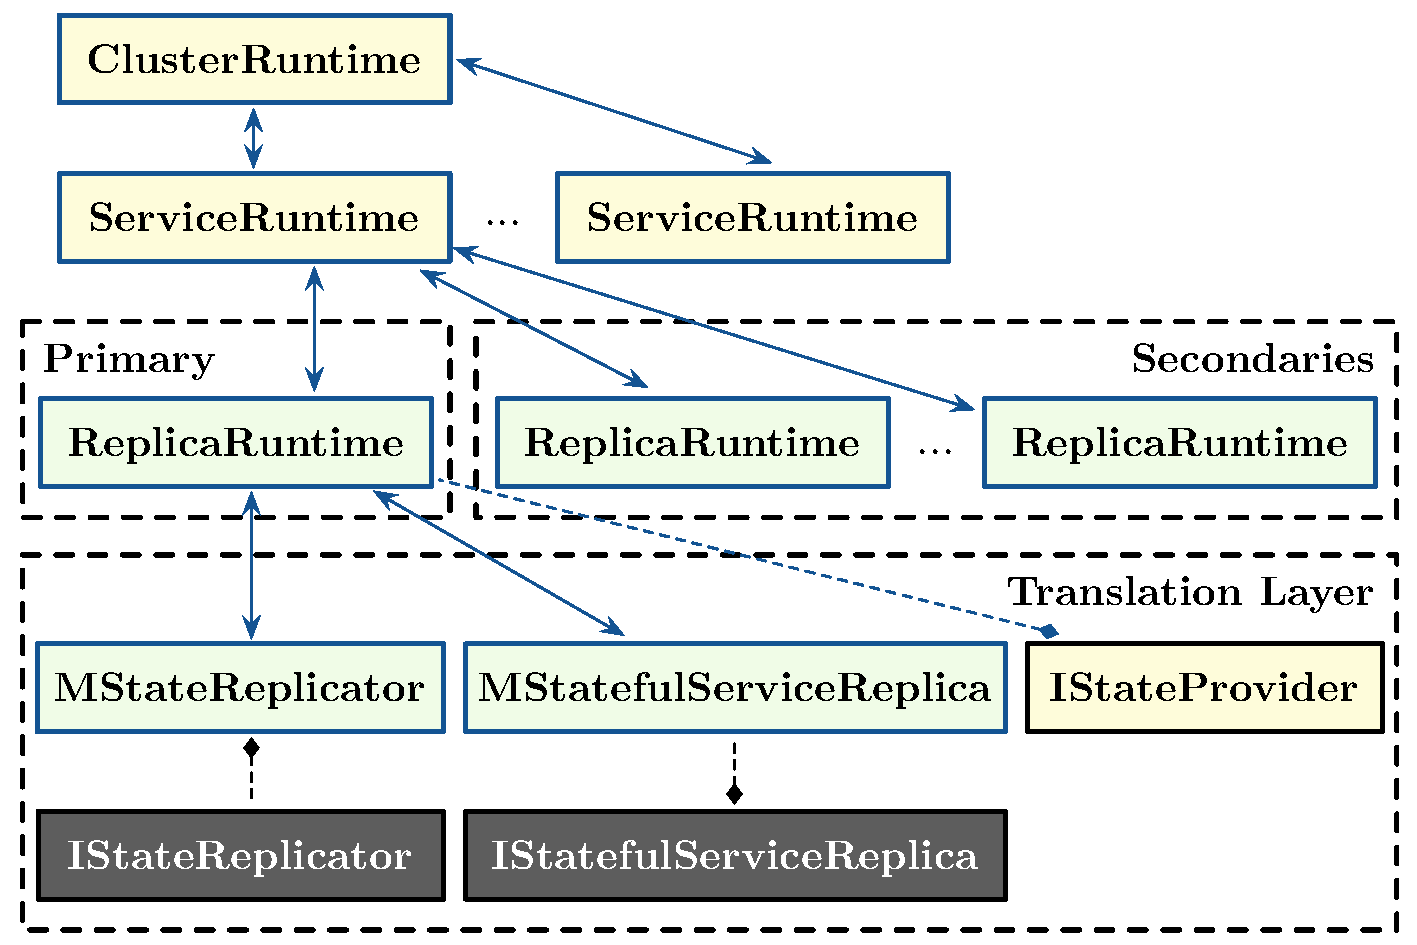
\includegraphics[width=\linewidth]{img/fabricmodel}
% \caption{Overview of the key machines and interfaces in our Fabric model.}
% \label{fig:fabric_model}
% \end{figure}

%\PTComment{Cut: overview of model.}
% An overview of our Fabric model is shown in Figure~\ref{fig:fabric_model}.
% The \texttt{ClusterRuntime} machine 
% handles the creation and management of 
% one or more Fabric services,
% as well as service resolution requests
% which allows for client-service and inter-service communication
% within the model.
% Each Fabric service instance is managed by a \texttt{ServiceRuntime}
% machine, which in turn manages 
% several \texttt{ReplicaRuntime} machines.
% Each \texttt{ReplicaRuntime} communicates with the user code
% via several machines and interfaces from the translation layer
% (only the translation layer for the primary is shown,
% but every \texttt{ReplicaRuntime} has its own instance of the translation layer).
% Note that communication between machines is hierachical;
% thus, communication between \texttt{ReplicaRuntime}s
% (such as the sending of replication requests)
% is via the \texttt{ServiceRuntime} machine for that service.
% This approach does not necessarily reflect how Fabric works in practice.
% Instead, we chose an architecture
% that keeps the model simple
% while still allowing (what we believe to be) realistic
% asynchrony and failure scenarios.

%\PTComment{Cut: Description of how replication works in the model, including how we modeled at a fine granularity.}
% \textbf{Replication example:} In order to replicate a state-mutating operation,
% user code at the primary replica 
% calls \texttt{IStateReplicator.ReplicateAsync},
% passing the serialized operation
% object.
% The operation is sent to the \texttt{ServiceRuntime},
% where it is assigned a \emph{logical sequence number} (LSN);
% each operation is assigned a consecutive LSN
% to track the total-order in which operations should be applied.
% The LSN is sent back to the primary replica
% where it is returned from the \texttt{ReplicateAsync} call,
% along with a \texttt{Task} object that will ``complete'' once
% the operation has been replicated to a majority of
% secondaries;
% thus, the user code can wait on the \texttt{Task}
% before confirming to any clients that the request has been applied reliably.
% The \texttt{ServiceRuntime} adds the operation to its list of in-flight
% replication requests and sends $n$ events to itself to signal that the request
% must be sent to a replica, where $n$ is the number of secondary replicas.
% The reason for sending $n$ events to itself instead of simply sending events
% directly to each secondary is so that the \texttt{ServiceRuntime}
% can process a simulated failure event inbetween the sending of replica requests
% to each secondary.
% This is an example of where we carefully considered
% the granularity of actions so that we could 
% model failures appropriately.
% The user code at a secondary receives the operation,
% applies it and then calls \texttt{Acknowledge} on the operation object;
% we implement this to send an event to the \texttt{ReplicaRuntime}
% which forwards the acknowledgement to the \texttt{ServiceRuntime}.
% Once a majority of secondaries have acknowledged, the
% \texttt{ServiceRuntime} removes the replication request from its list
% of replication requests
% and sends an acknowledgement to the primary,
% where the previously returned \texttt{Task} completes. 

%\PTComment{Cut: We reverse-engineered Fabric as needed.}
% \subsubsection{Fabric model correctness}
% Our model does not attempt to
% simulate the internals of Fabric accurately,
% as its purpose is to find bugs in user code
% and not in Fabric itself (which we assume to be correct).   
% However,
% due to lack of documentation,
% it is not always clear how Fabric should behave
% in certain scenarios.
% Thus,
% we ran several variants of a simple Fabric service
% that logs calls into the user code in order to
% reverse-engineer the actual behaviour of Fabric;
% we ensured that our model has the same behaviour,
% although this is an ongoing process as we encounter
% additional scenarios.

%\PTComment{Cut: We used systematic testing to find bugs in our model!}
% A further problem is that our model may contain bugs.
% In order to find bugs in our model effectively,
% we wrote a \psharp{} service made up of a single machine
% which takes the place
% of the user code and translation layer in Figure \ref{fig:fabric_model},
% for each \texttt{ReplicaRuntime}.
% Thus, we were able to run this pure \psharp{} system
% under \psharp{}'s systematic testing mode
% and uncover many assertion failures within our model.
% We tested a scenario where the primary fails at some non-deterministic point
% within the execution.

%\PTComment{Cut: Example bug found in our model plus the fix.}
% \textbf{Example Fabric model assertion failure:}
% In the buggy trace,
% the \texttt{ServiceRuntime}
% sends an \texttt{EEpochInfo} event to the second
% \texttt{ReplicaRuntime}
% indicating that this is the first epoch and the
% replica will be a secondary.
% An \emph{epoch} represents a configuration of primary and
% secondary replicas; when a different replica becomes the primary,
% this indicates the start of a new epoch.
% The \texttt{ReplicaRuntime} acknowledges that it has become
% a secondary by responding with the same event type.
% The \psharp{} service sends an \texttt{ESecondaryCopyContextOp};
% this indicates what state the secondary has
% and, thus, what the primary should send to this secondary so that it can catch
% up.
% The \texttt{ESecondaryCopyContextOp} event is forwarded to the
% \texttt{ServiceRuntime}. 
% The \texttt{ServiceRuntime} then receives and handles an \texttt{EKillPrimary}
% event, which causes the second replica to become the new primary.
% Thus,
% the \texttt{ServiceRuntime} sends another \texttt{EEpochInfo}
% to the second \texttt{ReplicaRuntime}
% indicating that this is the second epoch
% and the replica will be a primary.
% As part of this change,
% the \texttt{ReplicaRuntime}
% sends an event to the \psharp{} service
% indicating that it should stop waiting for
% the state to be copied from the old primary to this replica,
% which is acknowledged by sending an event to the \texttt{ReplicaRuntime}.
% This event causes the \texttt{ReplicaRuntime}
% to send an \texttt{ESecondaryCopyStateDone}
% event to the \texttt{ServiceRuntime},
% which unfortunately responds with an event indicating that the
% \texttt{ReplicaRuntime} is now an \emph{active} secondary
% (i.e.\ a secondary that has caught up with the primary).
% However, this causes an assertion failure because
% the \texttt{ReplicaRuntime} is becoming a primary and, thus,
% cannot be a secondary.
% Our fix to this bug was to ensure that the 
% \texttt{ESecondaryCopyStateDone} event was marked as part of the first
% epoch (as the \texttt{ReplicaRuntime} had not yet acknowledged the
% change to primary); thus, 
% the \texttt{ServiceRuntime} ignores the event and does not try to make the
% replica an active secondary.

% \subsubsection{CScale}

The main system that we tested using our \psharp Fabric model is \emph{CScale}~\cite{faleiro2012},
a big data stream processing system.
%In prior work~\cite{deligiannis2015psharp}, 
%we used an earlier version of the Fabric model and reported bugs in sample services.
Supporting CScale required significant additions to the model, making it much more
feature-complete.
CScale chains multiple Fabric services, which communicate via remote procedure calls (RPCs).
To close the system, we modeled RPCs 
using \texttt{PSharp.Send(...)}.
Thus, we converted a distributed system
that uses both Fabric and its own
network communication protocol
% that runs on the Fabric platform
% and 
% uses network communication
into 
a closed, single-process system. 
% that uses multiple threads,
% contains
% the Fabric model
% and the CScale services,
% and does not use network communication.
%\PTComment{Cut: we had to remove static fields.}
% Additional changes were needed to
% remove certain static (per-process) fields,
% as these were inadvertently
% being shared between services
% after making the system a single process.
A key challenge in our work was to thoroughly test CScale despite the fact that it
uses various synchronous and asynchronous APIs besides RPCs.
This work is still in-progress.
However, we were able to find a \texttt{NullReferenceException}
bug in CScale by running it against our Fabric model. The bug has been
communicated to the developers of CScale, but we are still awaiting a
confirmation.
